\section{Framework architecture}

\begin{figure*}
\centering
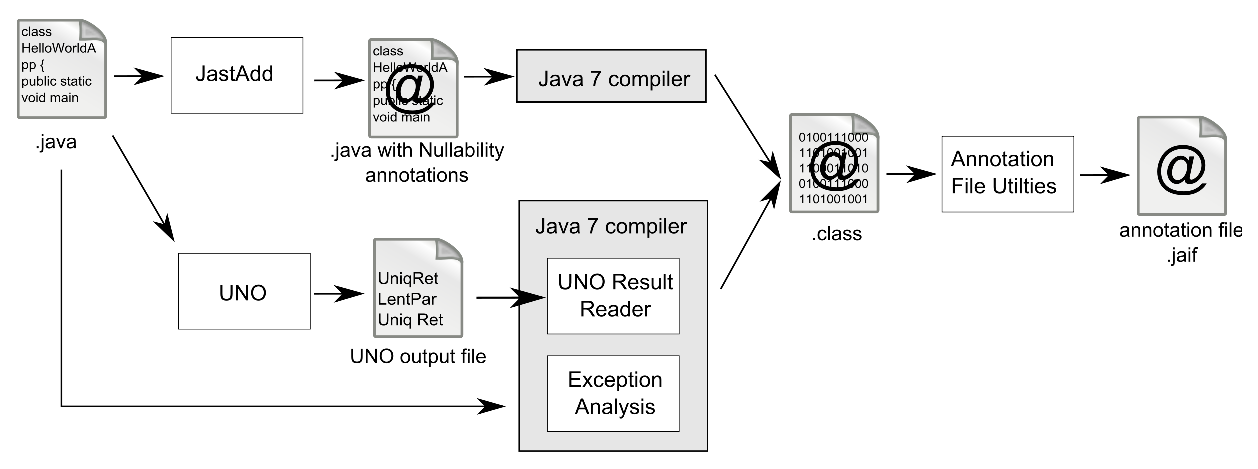
\psfig{file=figures/technicalApproach/from_source_to_jaif.eps, width=5.0in}
\caption{Toolchain from source to JAIF}
\label{fig:from_source_to_jaif}
\end{figure*}

To infer information about Java code we use two existing inference tools and 
an exception inference developed by ourselves and combine their output. 
Too aid in writing our own analyses, we have additionally developed a simple 
framework. 

To combine the results of disparate analyses we have to convert their results
into a common format.  We use the JAIF~\cite{JAIF}
(Java Annotation Index File) format for that purpose.  Some anaylses generate
results directly in JAIF format, some provide annotated bytecodes which can be
easily extracted into JAIF format, and others provide textual results for which
we will read the results into a our framework.

Figure~\ref{fig:from_source_to_jaif} 
illustrates the stages from the source to JAIF in our toolchain, explained 
below. While figure~\ref{fig:from_jaif_to_javadoc} shows how JavaGrok
puts the annotations back into the source files and generates the HTML
documentation.

In a first step JavaGrok inokes Uno to process the source code to annotate. 
Because Uno stores its inferred properties in a single separate file, 
we changed UNO's output format slightly to make it easier to parse it automatically.
To integrate the analysis results into the Java documentation we
use our own framework. We implemented a tree visitor inside the Java 7 
compiler that, at initialization, reads in the file generated by UNO and 
stores the information in a hashset. During the iteration over the AST
our visitor inserts annotation at the appropriate places. At the end of
this compilation the class files contain retention, uniqueness and exception 
annotations. These then get extracted into files in the JAIF format with the
help of the annotations file utilities AFU~\cite{AFU}.

% TODO: has to move into section 3: analysis
To infer exception annotation we use the Annotation Processing Tool (APT)
API~\cite{apt} built into the Java standard compiler.
% TODO: We will likely switch to also use the Type Annotation Processor! But not
% yet
From within an APT plugin
we can access the compiler's abstract syntax tree and augment the generated
bytecode with annotations representing our analysis results. These annotations
are then extracted into external annotation files.

JastAdd processes the source code and adds nullability annotations
directly into the source code. After that the source code with annotations
is compiled to class files which contain the annotations which again 
get extracted using the annotation file utilities.

Once the results of the various analyses have been collected into a set of
annotation files, the annotation file utilities~\cite{AFU} merge
those annotations back into the original source. The annotated source
code is now one of JavaGrok's output formats. Additionally Javadoc processes
the annotated source and combines the newly added annotations into the html
documentation.

\begin{figure*}
\centering
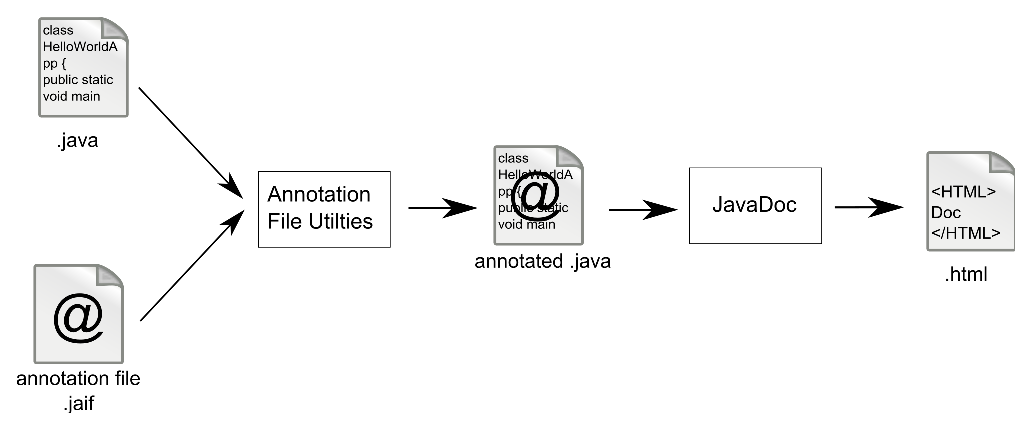
\psfig{file=figures/technicalApproach/from_jaif_to_javadoc.eps, width=5.0in}
\caption{From JAIF to Javadoc}
\label{fig:from_jaif_to_javadoc}
\end{figure*}